\begin{frame}{WebAssembly}
    \begin{itemize}
    \item WebAssembly: language virtual machine specification intended\ldots
        \begin{itemize}
        \item similar idea to Java VM
        \end{itemize}
    \vspace{.5cm}
    \item to be compiled to from C/C++
        \begin{itemize}
        \item support by Clang/LLVM
        \end{itemize}
    \item to be easy to just-in-time compile to native machine code
    \item to be run in web browsers (fast web apps)
    \end{itemize}
\end{frame}

\begin{frame}{WebAssembly memory management}
    \begin{itemize}
    \item WebAssembly `modules' have a single ``linear memory''
    \item starts at index 0, goes to some maximum
    \item load/store instructions take index into current memory
    \vspace{.5cm}
    \item observation 1: close to memory model ``normal'' C/C++ code expects
    \vspace{.5cm}
    \item observation 2: only goal is to prevent sandbox (WebAssembly) code from interfering with outside code
    \item \ldots so no need to check array bound or similar
    \vspace{.5cm}
    \item observation 3: no need to worry about garbage collection
    \end{itemize}
\end{frame}

\begin{frame}{WebAssembly validation}
    \begin{itemize}
    \item WebAssembly virtual machine code designed to be \textit{validated} before running
    \vspace{.5cm}
    \item allows for efficient interpreters or conversion to assembly
        \begin{itemize}
        \item validation ensures that you can safely skip certain type checks, etc.
        \end{itemize}
    \item language specification very explicit about what needs to be checked at runtime
    \end{itemize}
\end{frame}

\begin{frame}{example WebAssembly validation}
    \begin{itemize}
    \item check that instructions have right number of operands available
        \begin{itemize}
        \item WebAssembly instructions use stack (compile \texttt{2 + 2} into \texttt{2 2 +})
        \end{itemize}
    \item check operands that can be checked (constants)
    \item check the calls go to only functions listed in table
        \begin{itemize}
        \item should make it easier to do just-in-time compilation to machine code?
        \end{itemize}
    \item check the branches go to only locations listed in table, and only within one function
        \begin{itemize}
        \item should make it easier to do just-in-time compilation to machine code?
        \end{itemize}
    \end{itemize}
\end{frame}

\begin{frame}{example WebAssembly instruction specification}
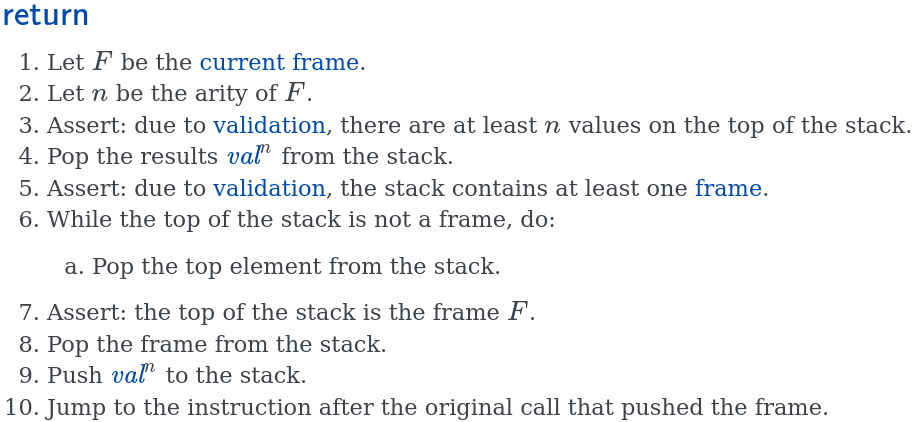
\includegraphics[height=0.8\textheight]{../sandbox/wasm-return-spec}
\end{frame}

\begin{frame}{WebAssembly as sandboxing}
    \begin{itemize}
    \item can compile existing C/C++ library using WebAssembly\ldots
    \item then call using language virtual machine
    \end{itemize}
\end{frame}
